%The remote system is composed by the remote server, that is a database, being connected to the local system in order to store its information. The remote server can be acessed by a remote client, which can be a web site or a mobile application. In this section is shown the system events, state charts and sequence diagrams of the remote client interface.

The remote system is composed by the remote server and remote clients: mobile application and web site. In this section are shown the remote system events, state charts and sequence diagrams.

\subsection{Remote Client}
\subsubsection{Mobile Application}
\paragraph*{Events}
In order to better understand the system, it is necessary to identify the events that may occur, how the system will respond to the event, what caused the event and what type of event it is. For the remote client mobile application, the events that may occur are presented in table \ref{table:rc_app_events}.

\begin{table}[ht]
	\centering
	\resizebox{\columnwidth}{!}
	{
		\begin{tabular}{|m{3cm}|m{5cm}|m{2.4cm}|m{2.4cm}|}
			\hline
			\textbf{Event} & \textbf{System Response} & \textbf{Source} & \textbf{Type}\\
			\hline\hline
			Login & Show application main screen if successful & Operator & Asynchronous\\
			\hline
			
			Obtain geolocation & Request device geolocation & Mobile device & Asynchronous\\
			\hline
			
			App notification & Notifies the operator about the lamppost status & Remote Server & Asynchronous\\
			\hline
			
			Register operator & Add operator information to \ac{db} & Operator & Asynchronous\\
			\hline
			
			Modify lamppost & Update lamppost information on \ac{db} & Operator & Asynchronous\\
			\hline
			
			Add new lamppost & Add new lamppost information to \ac{db} & Operator & Asynchronous\\
			\hline			
			
			Remove lamppost & Remove lamppost  from \ac{db} & Operator & Asynchronous\\
			\hline			
		\end{tabular}
	}
	\caption{Events: Remote Client Mobile Application.}
	\label{table:rc_app_events}
\end{table}

\paragraph*{Use Cases}
The mobile application use cases diagram are represented in figure \ref{fig:UseCases_application}, showing that the main actors in the system are the operator, the remote server and the mobile device. The operator can perform operations such as login, logout, register, modify information about a lamppost, remove a lamppost and register newly installed posts. For this, register a new installed post, the remote client acquires current device location from the mobile device and sends it to the remote server.

\begin{figure}[H]
	\centering
	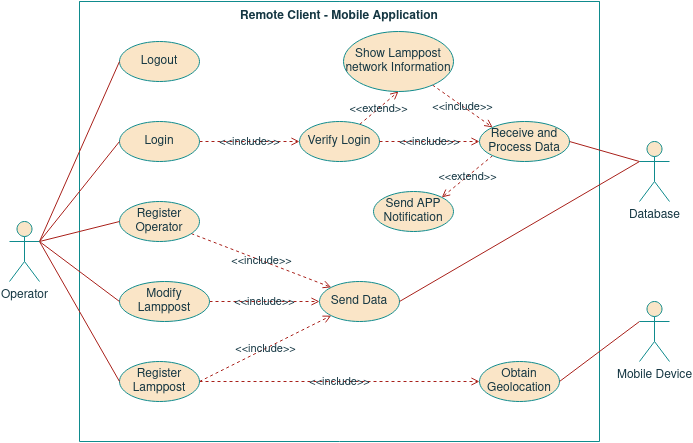
\includegraphics[width=1\textwidth]{06remote_system/AppSystem_UseCases}
	\caption{Use Cases: Remote Client Mobile Application.}
	\label{fig:UseCases_application}
\end{figure}

\paragraph*{State Chart}
In the figure \ref{fig:StateChart_application} is represented the state chart of the mobile application. It initiates with the system configuration, showing a home screen that allows the operator, the application user, to log into the system or register himself, if he doesn’t have login credentials. After a successful login, the system will show information about the lampposts associated to the logged in operator and he can do operations like register lampposts, remove lampposts, modify lampposts information and logout of the system.

\begin{figure}[H]
	\centering
	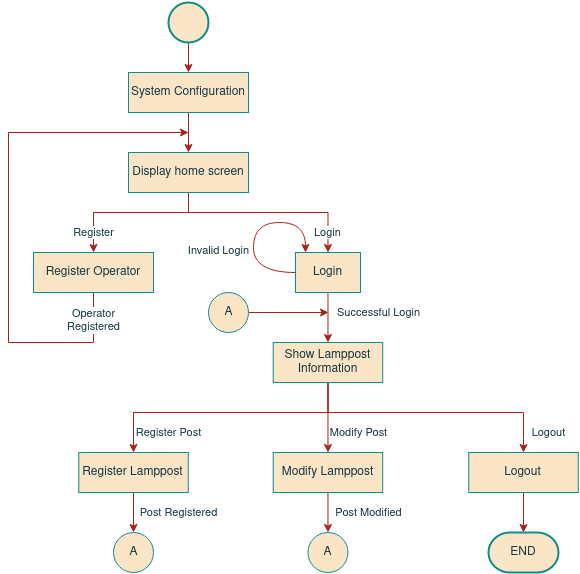
\includegraphics[width=1\textwidth]{06remote_system/AppSystem_StateChart}
	\caption{State Chart: Remote Client Mobile Application.}
	\label{fig:StateChart_application}
\end{figure}

\paragraph*{Sequence Diagram}
In figure \ref{fig:SeqDiagram_WebSite} is represented the sequence diagram of the mobile application. Most of the actions are triggered by the operator, starting with the registration or login operations in the application. If the login is valid, information about the network of lampposts will be shown and, depending on the interaction with the operator, the application may have different execution flows: registration of a lamppost; changing information about a lamppost or removing a lamppost; verification of the existence of damaged posts, notifying the operator if so. If the login is invalid, the application returns an error to the operator.

\begin{figure}[H]
	\centering
	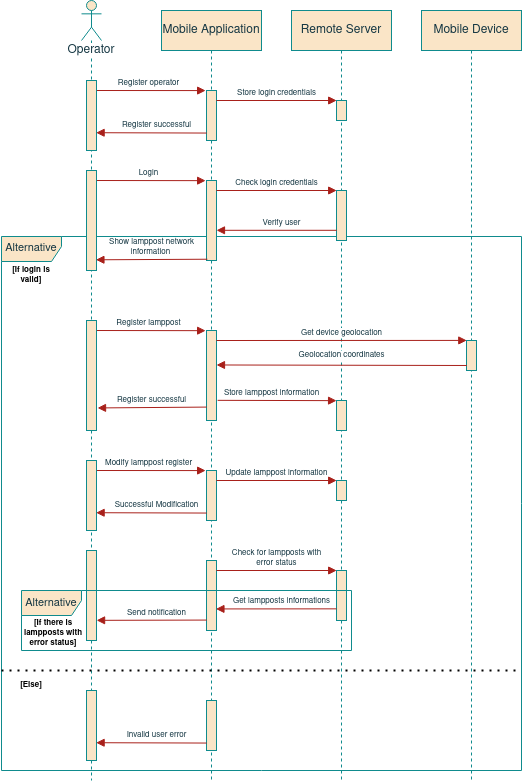
\includegraphics[width=0.90\textwidth]{06remote_system/AppSystem_SeqDiagram}
	\caption{Sequence Diagram: Remote Client Mobile Application.}
	\label{fig:SeqDiagram_application}
\end{figure}

\subsubsection*{Web Site}
\subparagraph*{Events}
In order to better understand the remote client web site, it is necessary to identify the events that may occur, which are presented in table \ref{table:rc_web_events}.

\begin{table}[ht]
	\centering
	\resizebox{\columnwidth}{!}
	{
		\begin{tabular}{|m{3cm}|m{5cm}|m{2.4cm}|m{2.4cm}|}
			\hline
			\textbf{Event} & \textbf{System Response} & \textbf{Source} & \textbf{Type}\\
			\hline\hline
			Insert location	& Show parking spots & User & Asynchronous\\
			\hline
			
			Obtain geolocation & Request device geolocation & Mobile Device & Asynchronous\\
			\hline
			
		\end{tabular}
	}
	\caption{Events: Remote Client Web Site.}
	\label{table:rc_web_events}
\end{table}

\subparagraph*{Use Cases}
The web site use cases are shown in figure \ref{fig:UseCases_WebSite}. The main actors are the user, the remote server and a mobile device. In order to know if there are available parking spaces in a certain location, the user can enter a location (inserting the street name, for example) or, as in the mobile application, use his mobile device to obtain the location automatically. The remote server lets the user know where there are empty parking spaces.

\begin{figure}[H]
	\centering
	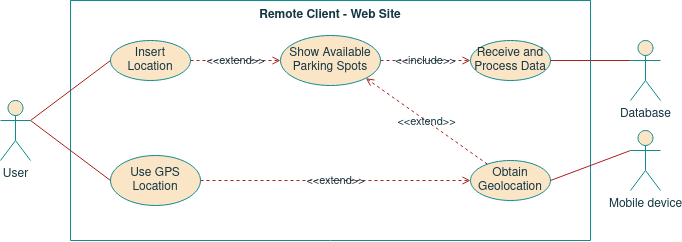
\includegraphics[width=1\textwidth]{06remote_system/WebSite_UseCases}
	\caption{Use Cases: Remote Client Web Site.}
	\label{fig:UseCases_WebSite}
\end{figure}

\clearpage
\subparagraph*{State Chart}
In figure \ref{fig:StateChart_WebSite}, one can see the web site state chart. The system initiates with the system configuration. Then the user can use his mobile phone's location (through the GPS tracking system) or type manually the location address. If the user enters a location manually (the street name, for example), it will be checked and, if valid, the available parking spaces will be displayed.

\begin{figure}[H]
	\centering
	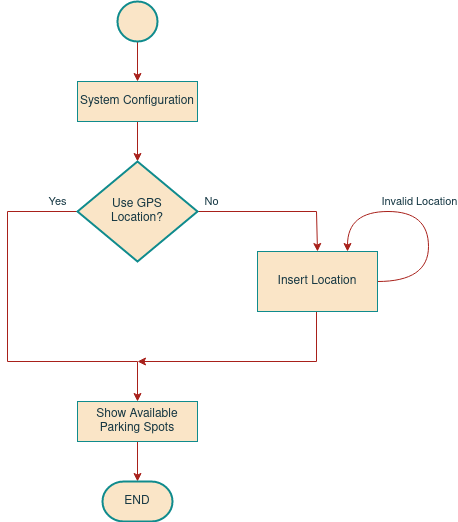
\includegraphics[width=0.8\textwidth]{06remote_system/WebSite_StateChart}
	\caption{State Chart: Remote Client Web Site.}
	\label{fig:StateChart_WebSite}
\end{figure}

\clearpage

\subparagraph*{Sequence Diagram}
The sequence diagram of the web site is shown in the figure \ref{fig:SeqDiagram_WebSite}. To know where there are empty parking spots, the user can insert manually a location or use his \ac{gps} location. In both cases the web site asks the remote server if there are available parking spots near the location and displays them to the user. However, in the case of using the \ac{gps} location, the web site has to get the \ac{gps} coordinates from the mobile device running the web site.

\begin{figure}[H]
	\centering
	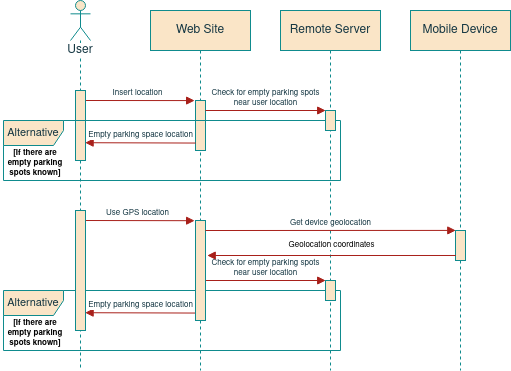
\includegraphics[width=1\textwidth]{06remote_system/WebSite_SeqDiagram}
	\caption{Sequence Diagram: Remote Client Web Site.}
	\label{fig:SeqDiagram_WebSite}
\end{figure}

\clearpage
\subsection{Remote Server}
\paragraph*{Events}
In order to better understand the remote server, it is necessary to identify the events that may occur, which are presented in table \ref{table:rs_events}.

\begin{table}[ht]
	\centering
	\resizebox{\columnwidth}{!}
	{
		\begin{tabular}{|m{3cm}|m{5cm}|m{2.4cm}|m{2.4cm}|}
			\hline
			\textbf{Event} & \textbf{System Response} & \textbf{Source} & \textbf{Type}\\
			\hline\hline
	
			Connection Request & Accept/ decline connection & Remote client & Asynchronous\\\hline
			
			Check Log-in Credentials & Validate username and pincode & Remote client (Mobile App) & Asynchronous\\\hline
			
			Add new lamppost & Add new lamppost info to \ac{db} & Remote client (Mobile App) & Asynchronous\\\hline
			
			Remove lamppost & Remove lamppost from \ac{db} & Remote client (Mobile App) & Asynchronous\\\hline
			
			Update lamppost information & Update lamppost info on \ac{db} & Remote client (Mobile App); Local System & Asynchronous\\\hline
			
			Check for lampposts with error status & Read and send lampposts with error status to Mobile App & Remote client (Mobile App) &  Asynchronous\\\hline
			
			Check for empty parking spots & Read and send available parking spots to Web Site & Remote client (Web Site) & Asynchronous\\\hline
		\end{tabular}
	}
	\caption{Events: Remote Server.}
	\label{table:rs_events}
\end{table}

\clearpage
\paragraph*{Use Cases}
The remote server use cases are shown in figure \ref{fig:UseCases_Server}. The remote(s) client(s) can interact with the remote server in various ways, as previously seen. This system only executes the demanded commands, from the remote clients or from the local systems, by accessing database information. The database interacts with the remote server by providing read, modify, remove or add register functions.

\begin{figure}[H]
	\centering
	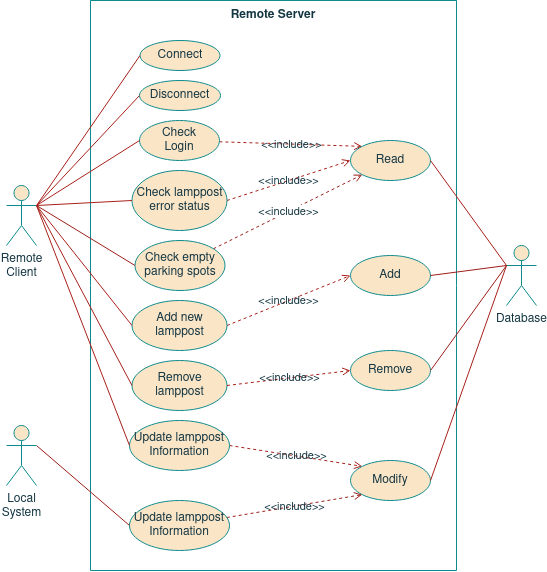
\includegraphics[width=1\textwidth]{06remote_system/Server_UseCases}
	\caption{Use Cases: Remote Server.}
	\label{fig:UseCases_Server}
\end{figure}

\paragraph*{State Chart}
In figure \ref{fig:StateChart_Server}, one can see the remote server state chart. After power on, the remote server does the system configuration, by initializing communication and database management services, and after that, the system executes concurrently these services until system's power off. These services give to the remote server the capability of processing received requests/commands, from the remote clients or from the local systems, and execute them, by accessing to database information.

\begin{figure}[H]
	\centering
	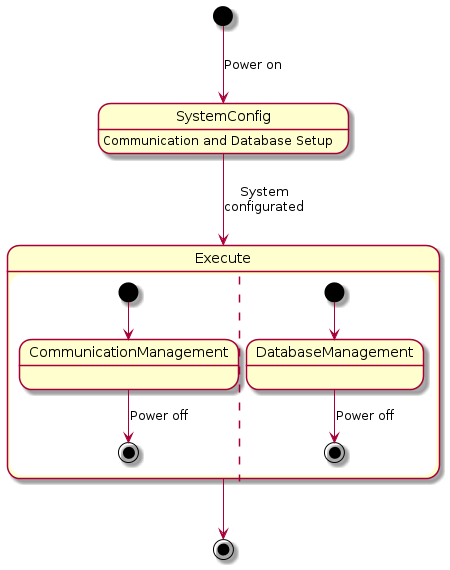
\includegraphics[width=0.8\textwidth]{06remote_system/Server_StateChart}
	\caption{State Chart: Remote Server.}
	\label{fig:StateChart_Server}
\end{figure}

\paragraph*{Sequence Diagram}
The sequence diagram of the remote server is shown in the figure \ref{fig:SeqDiagram_Server}. As seen previously, the remote client and the local system can execute several different actions. That is only possible if the remote server accepts the connection made from the remote client. After that, the remote server processes all received communications and, if needed, accesses the database to do so.

\begin{figure}[H]
	\centering
	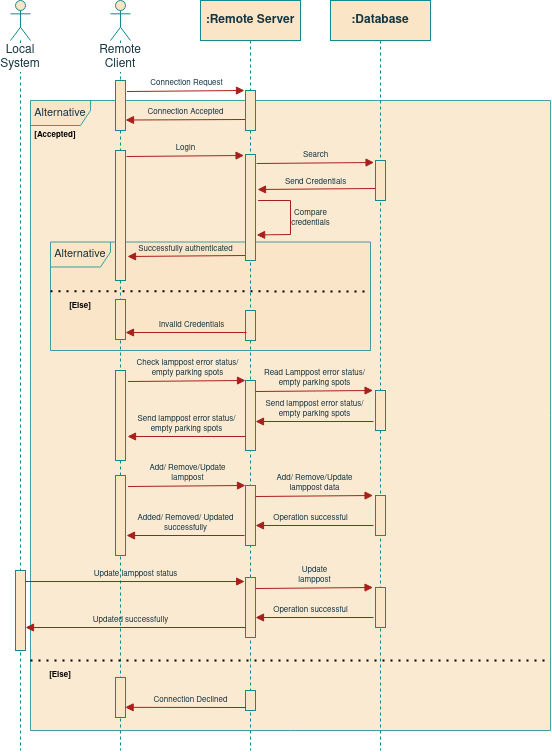
\includegraphics[width=1\textwidth]{06remote_system/Server_SeqChart}
	\caption{Sequence Diagram: Remote Server.}
	\label{fig:SeqDiagram_Server}
\end{figure}